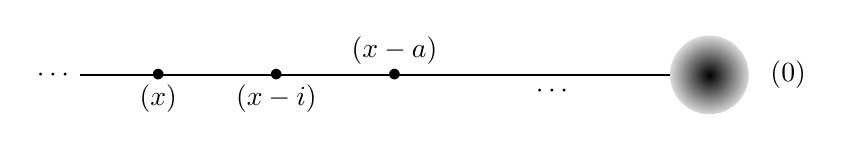
\begin{tikzpicture}
% Non-zero primes (closed points)
\draw[thick] (0,0) node[left] {\(\cdots\)}
    -- (1,0) node {\(\bullet\)} node[below] {\((x)\)}
    -- (2.5,0) node {\(\bullet\)} node[below] {\((x - i)\)}
    -- (4,0) node {\(\bullet\)} node[above] {\((x - a)\)}
    -- (6,0) node[below] {\(\cdots\)}
    -- (8,0);
% Generic point
\shade[inner color=black, outer color=gray!30]
    (8,0) circle (0.5);
\draw (9,0) node {\((0)\)};
\end{tikzpicture}